\section{Введение}
\label{sec:Chapter0} \index{Chapter0}

Известно, что разработка хороших, многоразово используемых библиотек является очень сложной задачей.
В популярных статических объектно-ориентированных языках, таких как Java и C++, наследование и подтипизация
(а в последнее время и обобщения в том числе) используются в качестве основных механизмов, способствующих многоразовому
использованию кода.
В то время как наследование позволяет одному классу повторно использовать реализацию
другого класса, например, объявления переменных и сигнатур методов, подтипирование предназначено для взаимозаменяемости.
Под взаимозаменяемостью подразумевается такое свойство сущности, что если объект одного типа может быть использован в
определенном месте, то и другой объект, являющийся его подтипом, также может быть использован в том же месте.
Взаимозаменяемость может быть также перефразирована как возможность повторного использования контекстов в том смысле,
что если некоторый контекст применим к объекту одного типа, то тот же контекст также применим к любому объекту его подтипа.
Для ясности дадим определения подтипа и супертипа.
Подтип - это тип, являющийся производным от другого типа, который называют супертипом.
Подтип наследует свойства и поведение своего супертипа, но также может добавлять дополнительные свойства или
переопределять существующие.
Подтипирование - это способ выразить, что один тип является специализированной версией другого.
Супертип предоставляет общее определение, которое может быть расширено или специализировано с помощью его подтипов.
Таким образом, проблемы проектирования, связанные с отношениями наследования и подтипирования, несколько различаются:
для наследования необходимо учитывать, как новые классы могут повторно использовать существующую реализацию,
а для подтипирования - как объекты могут использоваться в клиентском коде.

В популярных языках связь между подтипами по большей части основана на отношениях наследования.
Исключением являются только wildcards в Java 5.0.
Может случиться так, что два класса, используемые в схожих контекстах, но с довольно разными реализациями,
будут разделены в иерархии классов наследования, что приведет к отсутствию полезного супертипа этих классов.
Интерфейсы, как программная конструкция, в Java являются решением этой проблемы: можно определить суперинтерфейс
классов схожего назначения, независимо от заданной иерархии наследования, и пользоваться преимуществами подтипирования.
Однако интерфейсы не могут быть добавлены после определения класса, поэтому разработчикам библиотек по-прежнему
приходится много работать над планированием иерархий интерфейсов перед выпуском библиотеки в релиз.
Эта проблема считается существенным ограничением систем типов, основанными на взаимозаменяемости, как в Java.

В этой работе предлагается решение — объединение или union типы.
Union типы или объединения - это тип данных в некоторых языках программирования, позволяющий
переменной хранить значение, которое может быть одним из нескольких различных, в том числе
несвязанных между собой наследованием, но фиксированных типов.
Только один из типов, входящих в объединение, может быть ассоциирован с переменной в рантайме в
конкретный момент времени.
Они позволят решить проблему невозможности добавления супертипов к существующим типам, таким как классы и интерфейсы.

На практике различают два вида объединения - тегированный и нетегированный union.
Нетегированное объединение можно представить как фрагмент памяти, который используется для хранения переменных разных
типов данных.
Как только ему присваивается новое значение, существующие данные перезаписываются новыми данными.
Область памяти, в которой хранится значение, не имеет внутреннего типа (кроме просто байтов или слов памяти).
Однако это значение можно рассматривать как один из нескольких абстрактных типов данных, имеющий тип значения,
которое было последним записано в область памяти.
Нетегированные объединения обычно довольно ограничены в использовании и представлены только в не типобезопасных языках
программировании, таких как C\@.
Тегированное объединение можно рассматривать как тип с несколькими компонентами, каждая из которых должна быть
корректно обработана при манипулировании этим типом.
Говоря об объединении, по умолчанию будет подразумеваться тегированный union.

\begin{figure}
    \centering
    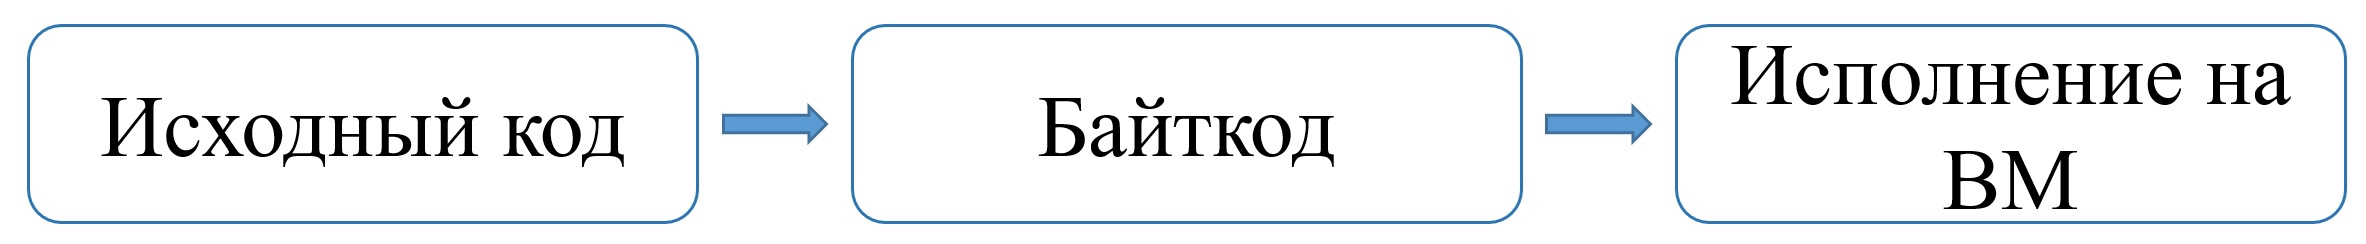
\includegraphics[scale=0.18]{Bytecode1.jpg}
    \caption{Общая схема исполнения программы}\label{fig:figure}
\end{figure}

Поскольку объединения состоят из существующих типов, они дают возможность определять супертип даже после того,
как иерархия классов установлена.
Как следует из названия, тип объединения обозначает объединение множества заданных типов, рассматриваемых как наборы
экземпляров, которые принадлежат к этим типам, и на уровне байткода и рантайма ведут себя как наименьший супертип.
Типы объединений могут использоваться не только при анализе вариантов, как в ML-типах данных, но и при прямом доступе
к элементам, как обычные типы.
Фактически, для некоторых типов их объединяющий тип можно рассматривать как интерфейс,
который "выделяет" их общие черты, то есть поля с одинаковыми именами и методы с похожими сигнатурами.
Мы ожидаем, что объединяющие типы могут быть полезны для группировки независимо разработанные классы со схожими
интерфейсами, с указанием их супертипа, а также для реализации гетерогенных коллекций, таких как списки, в которых,
скажем, строки и целые числа смешаны в качестве элементов.


todo: описать боксинг анбоксинг

\newpage
